% Template for PLoS
% Version 1.0 January 2009
%
% To compile to pdf, run:
% latex plos.template
% bibtex plos.template
% latex plos.template
% latex plos.template
% dvipdf plos.template

\documentclass[10pt]{article}

% amsmath package, useful for mathematical formulas
\usepackage{amsmath}
% amssymb package, useful for mathematical symbols
\usepackage{amssymb}

% graphicx package, useful for including eps and pdf graphics
% include graphics with the command \includegraphics
\usepackage{graphicx}

% cite package, to clean up citations in the main text. Do not remove.
\usepackage{cite}

\usepackage{color} 

% Use doublespacing - comment out for single spacing
%\usepackage{setspace} 
%\doublespacing


% Text layout
\topmargin 0.0cm
\oddsidemargin 0.5cm
\evensidemargin 0.5cm
\textwidth 16cm 
\textheight 21cm

% Bold the 'Figure #' in the caption and separate it with a period
% Captions will be left justified
\usepackage[labelfont=bf,labelsep=period,justification=raggedright]{caption}

% Use the PLoS provided bibtex style
\bibliographystyle{plos2009}

% Remove brackets from numbering in List of References
\makeatletter
\renewcommand{\@biblabel}[1]{\quad#1.}
\makeatother


% Leave date blank
\date{}

\pagestyle{myheadings}
%% ** EDIT HERE **
\newcommand{\COMMENT}[1]{{\color{red} #1 }}
\newcommand{\COM}[1]{{\color{blue} #1 }}

\graphicspath { {./figures/fig1/} {./figures/fig2/} {./figures/fig9/} {./figures/fig5/}}
\usepackage[normalem]{ulem}
\usepackage{amssymb}
\usepackage[colorlinks]{hyperref}
\usepackage{booktabs}
\usepackage{amsmath}
%\usepackage{multirow}% http://ctan.org/pkg/multirow
%\usepackage{tablefootnote}
%\usepackage{import}
\usepackage{subcaption}
\usepackage{caption}
%\usepackage[format=hang,font=small,labelfont=bf]{caption}


%% ** EDIT HERE **
%% PLEASE INCLUDE ALL MACROS BELOW

%% END MACROS SECTION

\begin{document}

% Title must be 150 characters or less
\begin{flushleft}
{\Large
\textbf{A quantitative assessment of the Hadoop framework for analyzing massively parallel DNA sequencing data}
}
% Insert Author names, affiliations and corresponding author email.
\\
Alexey Siretskiy$^{1 \ast}$, 
Luca Pireddu$^{2}$, 
Ola Spjuth$^{3,4}$
\\
\bf{1} Department of Information Technology, Uppsala University, Uppsala, Sweden
\\
\bf{2} CRS4, Polaris, Pula, Italy
\\
\bf{3} Department of Pharmaceutical Biosciences, Uppsala University, Uppsala, Sweden
\\
\bf{4} Science for Life Laboratory, Uppsala University, Uppsala, Sweden
\\
$\ast$ E-mail: alexey.siretskiy@it.uu.se
\end{flushleft}

% Please keep the abstract between 250 and 300 words
\section*{Abstract}
New high-throughput technologies such as massively parallel sequencing has transformed the life sciences into a data-intensive field. With increasing data volumes comes the necessity to analyzee data in parallel using high-performance computing resources, but doing this effectively can be laborious and challenging. 
Hadoop, emerging in the last decade, is a framework that automatically distributes data and computation and has been shown to scale to thousands of nodes. Herein we introduce metrics and report a quantitative comparison of Hadoop to regular high-performance computing resources for aligning short reads and calling variants for five datasets of different sizes up to 250\,gigabases. In order to increase performance of existing software and obtain a better comparison we modified and wrote new analysis scripts. From the observed scaling relations we are able to draw conclusions about the perspectives of the approaches, leading to the conclusion that as data set sizes reach 100\,gigabases, the Hadoop-based pipelines become performance-competitive with a canonical high-performance cluster solution. As data sets in biological sequencing are sure to increase with time, Hadoop and similar frameworks are very interesting technologies that we envision will play a key role in the future of biological data analysis.

% Please keep the Author Summary between 150 and 200 words
% Use first person. PLoS ONE authors please skip this step. 
% Author Summary not valid for PLoS ONE submissions.   
\section*{Author Summary}
New experimental technologies generate vast amounts of data and require supercomputers to store and analyze. As datasets increase in volume there is a need for new computational tools and technologies that can cope with the scale of data, and in this paper we provide a detailed study comparing the performance of the Hadoop framework with traditional high-performance computing for data in biological sequencing. While there is an overhead of using Hadoop, we show that when sequencing data sets reach sizes of 100 gigabases then Hadoop becomes attractive compared with traditional methods. We also show that Hadoop scales linearly while traditional systems become network-saturated at larger data sizes. As sequencing data are bound to increase in the future, Hadoop is a very interesting framework to base future analysis on.




%%%%%%%%%%%%
% Introduction
%%%%%%%%%%%

\section*{Introduction}
%The problem: dealing with BIG data
Since its inception, massively parallel DNA sequencing, also referred to as Next Generation Sequencing~(NGS) technology, has been an extremely bountiful source of data giving insight into the workings of biological machinery~\cite{metzker, Marx:2013fk}. Decreasing sequencing costs facilitates and promotes larger and larger studies with increasingly larger data sizes, and extracting useful information from these voluminous amounts of data is transforming biology into a data-intensive discipline that requires a high-performance computing (HPC) infrastructure to analyze.  As an example of the scale of the demands, consider that a single Illumina high-throughput sequencing run produces approximately 1800\,gigabases (Gbases) corresponding to 2\,terabytes (TB) of raw data in 3 days~\cite{illumina}.

%Current practices: HPC systems
A common step of NGS data analysis consists of alignment short reads to a reference sequence and then finding the genetic variations specific to the sample.
Many of the most widespread tools for this purpose, like BWA~\cite{bwa}, Bowtie~\cite{Langmead:2009uq} and Samtools~\cite{samtools}, are not made with distributed computing in mind. Many others do not even have the native ability to use multiple cores. 

%Current practices: How to parallelize
The most common approach to speed up NGS tools is to parallelize within a compute node (multi-core parallelization) using shared memory parallelism~(OMP)~\cite{openmp}, but this approach is naturally limited by the number of cores per node, which does not usually exceed~16, see~\cite{top500}. For the tools which do not support OMP natively, e.g. Samtools, variant calling can be parallelized by creating a separate process  for  each chromosome, or using GNU Parallel Linux utility~\cite{Tange2011a}.
Of great importance is that a multi-core approach does not improve the performance of operations that are limited by local disk or network throughputs, whereas splitting the dataset and multi-node parallelization generally are not bound by these constraints.

Message Passing Interface~(MPI)~\cite{mpi1} is a common way to implement multi-node parallelization, but writing efficient MPI-programs for hundreds of cores is a non-trivial task since thread synchronization (or load balancing) has to be woven into the software code and there are few existing solutions available for processing sequencing data~\cite{pmap, erne, gnumap}.

Another common way to introduce parallelization to NGS analysis pipelines in Linux systems is to use Bash scripting. This involves using existing utilities and cluster tools to split the data into chunks, process them on the separate nodes, and merge the results afterwards. This kind of solution benefits from both MPI-like and OMP parallelization and provides good performance, but the development requires substantial expertise in order to be efficient. Since the process is tightly coupled to the local computational cluster and network architectures, it might also not be possible to be re-used in other settings.

%Introduce Hadoop, MR, and HDFS
%Properties of Hadoop and HDFS- data localization and programming model etc
The Map-Reduce~(MR) programming paradigm~\cite{hadoop} offers a compelling alternative for running tasks in a {\it massively} parallel way. This paradigm, however, shifts the focus from the best performance to scalability, suited for managing huge datasets of sizes up to several terabytes~\cite{lin2010}.
The most prevalent open source implementation of Map-Reduce is Hadoop~\cite{hadoop,Hadoop:Guide}.
The Hadoop~MR framework provides automatic distribution of computations over many nodes as well as automatic failure recovery (failure of individual jobs or computing nodes by storing multiple copies on different nodes), and automated collection of results~\cite{Hadoop:Guide}. Hadoop Distributed File System~(HDFS) is a complementary component that stores data by automatically distributing it over the entire cluster, writing data blocks onto the local disk of each node and therefore effectively moving the computation to the data and reducing network traffic. HDFS provides a storage system whose bandwidth and size scales with the number of nodes in the cluster~\cite{Sammer:2012}, which is very different from the properties of the usual HPC cluster network architecture. 

%Manuscript focus: When is Hadoop currently an appealing alternative
%Introduce what we did in the manuscript.
In this manuscript we focus on the question {\it when} Hadoop is an appealing alternative to the program tools generally found in~HPC centers for DNA-seq analysis. 
Since Hadoop is written in Java, which is slower than the standard~HPC programming languages like C or Fortran, we seek to estimate an average data size when it starts to be worthwhile to use Hadoop from a performance perspective. We also study execution times for datasets of different sizes and analyze Hadoop and HPC approaches from a scaling perspective.


%%%%%%%%%%%%
% Results
%%%%%%%%%%%%
% Results and Discussion can be combined.
\section*{Results}

We constructed two pipelines for identifying single-nucleotide polymorphisms (SNPs) from short read data, one based on Hadoop and the other on regular HPC with a batch processing system (hereafter referred to as HPC method) (Methods). 
Our experiments then consisted of running the pipelines for five datasets with short reads of different sizes and measuring the wall-clock run time for each pipeline stage. 
All experiments were repeated several times and the results averaged to obtain a data point for the particular combination of data size and computational platform.
For the existing Hadoop software we propose modifications, in order to benefit fully from massively parallel nature of MR computations.
For the classical HPC DNA-seq analysis programs we developed a set of Bash scripts utilizing multiple nodes for short read alignment and exploiting the network fully, thereby speeding up calculations.



\subsection*{Modified preprocessing stage}
A native preprocessing stage in Crossbow provides great flexibility in delivering the data to the Hadoop cluster, where data can be downloaded from Amazon S3, FTP and HTTP servers over the Internet~\cite{Langmead:2009kx}. The only way to introduce parallelization in the native preprocessing stage is to split the read files into smaller chunks and to generate a manifest file listing all these chunks. This, however, is lacking the massively parallel way of treating the data.

%\footnote{the same holds for Myrna, a cloud-based solution for differential expression analysis} 

Assuming that sequencing platforms are usually in close proximity with facilities that provide both storage and computers, we considered that the data already had been downloaded to storage that Hadoop could access.
We rewrote the Crossbow preprocessing stage scripts in a MR-manner, benefiting from its massively parallel nature.
The requirement is that the FASTQ data are i.e. BZIP2 archived (however, any splittable archive format is suitable) and accessible by Hadoop. For our case the storage with the data was mounted with SSHFS to one of the Hadoop nodes, from where the BZIP2'ed data were transferred to the HDFS.
BZIP2 provides very good compression and is splittable, meaning that the archive can be expanded in a parallel manner. Also, BZIP2 format is natively supported by Hadoop, i.e., there is no difference in dealing with the FASTQ data or with its BZIP2 archive.

%\footnote{other options like splittable LZO are also possible}

The Hadoop streaming library offers a possibility to write code for Hadoop jobs in any programming language. Our Python scripts efficiently process short reads, produced by Illumina sequencing platform of different versions, as well as the FASTQ files converted from SRA format (NCBI Sequence Read Archive~\cite{ncbi-sra}).
The problem of lacking the unique FASTQ header standard was solved by the rewriting the header based on a SHA-1 hash function, and the reads mates were labeled with ``.1" and ``.2" suffixes. 
To ensure that both the forward and reverse reads of the same pair would end up on the same Reducer, secondary Mapper key-sorting mechanisms were involved.

In order to compare the native preprocessor and the proposed one, the data was put on HDFS beforehand to eliminate possible network delays, e.g., while downloading data from Amazon.
Table~\ref{table:preprocess} illustrates the benefits of our approach.
To complete the comparison the same preprocessing was performed with a BASH script for the same data located on the HPC storage. The script utilizes multiple cores and was executed on a single HPC node (see Supplementary information).
%ran on a single HPC node, utilizes multiple cores, with the limiting factor being \sout{the hard disk IO performance.}\COM{More correctly to say, that the pipe is not filled completely. i.e. the degree of achieved parallelization does not utilize all 16 cores. Perhaps not the best bash commands etc.}
%, which effectively leaves with 5-7 cores of 16. \COMMENT{awkward}


\subsection*{Accuracy of pipelines}
Since our HPC and Hadoop approaches use different~SNP callers (Samtools and SOAPsnp, correspondingly) we should not expect them to deliver perfectly matching SNP lists, but still we expect them to capture and correctly identify the mutations. We tested the correctness just for the smallest dataset~(I). The mutation $C\rightarrow T$ on chromosome 4 at position $16702262$\cite{schneeberger} was successfully localized by both applications.



\subsection*{Scalability of HPC and Hadoop approaches}
To demonstrate the scalability of the HPC approach we collected running times for dataset~I as a function of the number of cores used (Table~\ref{table:3}). 
The alignment process in Bowtie scales fairly well, but the SNP calling part in Samtools is a bottleneck, scaling worse than Bowtie, and consuming a progressively larger portion of the total calculation time even after parallelizing analysis by chromosome as previously suggested~\cite{biostars_samtools}.
%\footnote{\url{http://www.biostars.org/p/48781}
%\COM{here was a footnote referring to biostars site. Ok, if the footnotes are not welcome, lets then have it as a reference. That code is not trivial. Maybe we can leave the ref?}
%\footnote{The amount of available memory, specified with the \texttt{-m} option, is of big importance for the Samtools performance. During its sorting phase the lack of RAM results in spilling to the HDD. For example for an half of  Dataset III, SNP calling takes approximately 40 minutes with 8 GB RAM, and 15 minutes with 48 GB RAM, when  the whole BAM file fits into RAM. For our tasks we used the default Samtool's settings.}.  
For the given datasets (I--V) the timings for alignment against the corresponding genomes and SNP calling for the HPC and Hadoop approaches were collected (Table~\ref{table:4}).

One of the attractive sides to run i.e. Samtools, Bowtie, etc. in the  Hadoop~MR framework is its almost linear scalability, i.e., calculation time linearly depends on the size of the dataset\cite{Langmead:2009kx,Pireddu:2011vn}, regardless the scaling nature of the underlying program.
Figure~\ref{fig:fig1}, based on Table~\ref{table:4}, shows the calculation time as a function of the dataset size for the 56 cores Hadoop cluster and datasets I-IV.
%To stress the linear nature of scaling, both sets of points were fit using the least squares method.



\subsection*{Comparing Hadoop and HPC runtime efficiency}
Hadoop was designed to digest huge datasets\cite{hadoop,lin2010}. One can propose then that the larger the dataset is, the more suitable Hadoop becomes compared to the HPC approach. In order to compare the ``suitability'' for different types of calculation platforms (Hadoop and HPC) each being run on a different number of cores, we constructed the function showing the amount of used core-hours:
$F=T_{p}\times p,$ 
where~$T_{p}$ is the calculation time on~$p$ cores. 

Using the data from Table~\ref{table:4}, we plot the ratio $F_{Hadoop}/F_{HPC}$ as a function of the reciprocal dataset size (Figure~\ref{fig:fig2}). Extrapolation to zero on the~$X$-axis estimates the ratio for the hypothetical infinite dataset. As one can see, the Hadoop approach becomes more and more effective compared to the HPC scenario as the dataset size increases. 
The parabolic extrapolation for our settings give the ratio as~$1.70\pm0.01$, meaning that Hadoop running even in the virtualized environment of a private cloud assembled on moderate hardware, is competitive with the HPC approach run on ``bare metal'' of modern hardware for datasets greater than $100$\,Gbases (dataset~IV), which is typical for human genome sequencing with a sequencing depth of about~$30x$.


The simplest curve to fit the points nicely is a parabolic function, importantly not a constant. 
Since the Hadoop approach for the datasets reveals the linear scaling (Figure~\ref{fig:fig1}), a deviation of the ratio from the constant shows the 
lack of scalability of the HPC approach.
%Consider the linear scaling for the Hadoop approach for the same datasets, we conclude that HPC approach scales worse than linearly.
%\footnote{For the linear scaling the curve of $F=T_{p}\times p$ does not depend on the dataset size, i.e. being a constant; thus the ratio of two constants would result a constant, but we observe a dependecy.}. \COMMENT{Why jump back and forth in the discussion of figures 1 and 2?} 
We suspect the main reason for such a behavior is the fact that for large datasets (dataset~III-V in our case) the SNP calling routine with Samtools becomes more memory and time demanding than the actual alignment with Bowtie.
If lacking RAM, Samtools  swaps to disk, creating multiple (up to hundreds) temporary files while sorting the BAM file, keeping the network load for NFS storage and time-expensive IO on a high rate.
Table~\ref{table:5} shows the sorting runtime performance of Samtools for the dataset~IV run with different amount of RAM available on a single HPC node. The large uncertainty for small amounts of RAM we believe is due to other users' load on the cluster network. As a result, a large amount of RAM per node is needed in order to use Samtools effectively, while Hadoop accomplishes SNP calling on much more economic hardware in linear time with just 12GB RAM per virtual node.


 \subsection*{Comparing the network communication efficiency for the Hadoop and HPC approaches }
The network communication model for Hadoop has a major difference from the usual HPC cluster network architecture ($n$-tier tree) with NAS or NFS attached storages. The effective bandwidth of the Hadoop network increases with the cluster size~\cite{Sammer:2012}, opposite to that of the HPC network where cluster growth results in network saturation and performance depletion.
To study this phenomena, we compared HPC and Hadoop network communication costs depending on the number of nodes involved for a fixed dataset size (58~Gbases, dataset~IV).
 
Due to the trivially parallelizability of the alignment process~-- the read-pairs are independent of each other, and can be aligned independently~-- one could try to involve more computational resources, e.g., split the initial data into chunks to process them independently.
Reducing the size of each data chunk reduces the aligner  job,~$T_{alignment}$, but at the same time, the more chunks almost simultaneously have to be sent over the network, potentially causing traffic jams, and therefore increasing the communication costs,~$T_{comm}$.

There are several program packages for short read alignment with MPI support~\cite{pmap, gnumap}, and almost linear scaling up to 32 nodes for pair-ended reads has been reported~\cite{Bozdag:2010cn}. However, e.g., the Pmap package functions poorly for datasets larger than 20 Gbases. To circumvent this limitation we implemented a highly optimized Bash script making use of standard Unix utilities to use the HPC cluster network as efficiently as possible~\cite{code_repo_bash}, and compared the network performance with the standard Hadoop HDFS approach. We separated the alignment time, $T_{alignment}$, and the communication time, $T_{comm}$, and plotted $T_{alignment}/T_{comm}$ as a function of the reciprocal number of nodes~$1/N$ (Figure~\ref{fig:fig3}). 
This measure is applicable to both HPC and Hadoop, however, $T_{comm}$ has a different explanation. For Hadoop, the short reads in FASTQ format have to be preprocessed (involving node communication~$T_{comm}$) to be able to run in MR-fashion, while the data locality will be automatically achieved during the data ingestion into the HDFS. 
We rewrote the code for the preprocessing stage for Crossbow to make it suitable for MR-style parallelization.
For the HPC approach, $T_{comm}$ involves the chunks that are sent from the sequence delivery location to the local node scratch disks where the actual alignment happens, and the sending of the aligned SAM files back to the delivery location over the network.
%\footnote{\url{http://samtools.sourceforge.net/SAMv1.pdf}}

%The HPC approach is presented in two versions that are based on a bit different strategies of the resource allocation.  

\textit{Hadoop results (filled circles in Figure~\ref{fig:fig3})}: One can see that the ratio~$T_{alignment}/T_{comm}$ reveals very weak dependency in a wide range of number of nodes~$N$: from 4 up to 40. It is known that Bowtie provides almost linear scaling between alignment time and dataset chunk size~$D$:~$T_{alignment}\propto  D\propto 1/N$, see~\cite{Langmead:2009uq}, and Figure~\ref{fig:fig1}. Since the ratio~$T_{alignment}/T_{comm}$ is approximately constant, one can conclude that $T_{comm}\propto 1/N$, meaning that the more nodes involved, the faster the communication is in the preprocessing stage.

%The strategy named HPC SLURM\footnote{Simple Linux Utility for Resource Management}   is as follows: 
\textit{HPC results (open circles in Figure~\ref{fig:fig3})}: The data from the delivery location is split into chunks in parallel, which are simultaneously pushed to the local scratch disks of the nodes allocated by SLURM. One can see two distinct linear stretches. One stretch is for the range from 4 to about 12 nodes, and the another is from 12 up to 60. The former (horizontal stretch) is explained as for Hadoop~-- the more nodes involved, the faster the chunks are being distributed. The latter stretch with the positive slope could be explained as follows: In the region of about 12 nodes the network becomes saturated
%\footnote{The used storage at UPPMAX is a set of RAIDs (Redundant Array of Inexpensive Disks) with data striping, providing up to $80$Gbasesit/sec of outcoming traffic \COMMENT{'outgoing' or 'incoming' or just 'traffic'}.} 
and unable to pass more data in a time unit, while the alignment time is still proportional to the chunk size:~$T_{comm}\approx\mbox{const}, T_{alignment}\propto D\propto 1/N \rightarrow T_{alignment}/T_{comm}\propto 1/N$, i.e., a linear dependency, which can be observed in the plot. 
The transition area between the two modes is based on the fact that each hard disk drive on the local node can write the data at a speed of about 1Gbit/sec. Ten nodes will consume the data with the rate of~10Gbit/sec, which is the limiting speed for the standard 10Gbit Ethernet cable connecting the cluster's rack with the switch. The nodes are being allocated on the same rack, which is the default SLURM behavior.

Scalability can be improved by overriding the default behavior of SLURM and allocating the nodes not from the same rack, but randomly from all available racks (``HPC random'', open squares in Figure~\ref{fig:fig3}). Allocating the nodes on random racks allows one to engage more nodes without network saturation. For our cluster we could go up to 30-35 nodes with perfect linear scaling. For the most resources used (58 nodes) the deviation from a linear speedup is~$\approx 7\%$ i.e. $5.50$ minutes against the ideal $5.14$, see Table~\ref{table:4}. The threshold number of nodes in this strategy~($\approx35$) is because of the uplink cable with the throughput of~50Gbit/sec being saturated. 
The proposed HPC strategies aimed at getting the maximum performance from the storage resources show that while even properly adjusted and tuned, the HPC approaches suffer from the network saturation at higher number of nodes.
HDFS on the other hand maintains data locality, reducing communication and data transfer and hence lead to better scalability.
Our Hadoop cluster has no more free nodes to continue to investigate the scaling as in plot at Figure~\ref{fig:fig3}, but we do not expect any significant deviations, since the observed behavior is a generic for Hadoop with HDFS\cite{lin2010, Hadoop:Guide}. 


\subsection*{Usability aspects}
\label{subsectionIV_2}

A popular way to construct and execute bioinformatic pipelines on HPC resources is via the Galaxy\cite{galaxy} platform, which provides a Web-based graphical user interface~(GUI) to bioinformatic programs, simplifying the experience for the end user. 
An alternative for Hadoop is Cloudgene\cite{cloudgene}, which is a light-weight and flexible Web-based solution for both public and private clouds. We implemented our Hadoop-pipeline in Cloudgene and extended the platform with functions to import data from the central file system at UPPMAX into HDFS on the private cloud (Figure~\ref{fig:fig4}).
For our particular task in DNA sequencing, Cloudgene makes it easy to select data and parameters for its execution. Most of the data managing work is done automatically and the results can be downloaded to the client machine. The modular structure allows modification of the source code to adapt to the existing computing center architecture. For example, UPPMAX users can import their data from the sequencing platform directly to the Hadoop cluster by pressing a button and entering the credentials, being at the same time sure that their sensitive data is kept privately.





%%%%%%%%%%%%
% Discussion
%%%%%%%%%%%%
\section*{Discussion}

In this report we have described two approaches for high-performance analysis of DNA sequencing data; one based on regular HPC using a batch system and one based on Hadoop. We show that Hadoop installed on a private cloud is an appealing solution both on terms of runtime performance and also in terms of usability. A key result is the data size where Hadoop is favorable to regular HPC batch systems, and in order to compare them we developed highly optimized pipelines for both scenarios. We found that dataset sizes larger than 100\,Gbases is where Hadoop excels over HPC, and also that Hadoop shows almost linear scalability for this problem. Extrapolation to infinite dataset size reveals however that HPC provides the results faster, given the same amount of resources as Hadoop on a private cloud.

We modified the preprocessing stage of the Crossbow software to enable it to make use of all nodes in the Hadoop system, end used a highly optimized Bash script to compare the scaling relations between the ratio of the alignment time to the communication time as a function of the reciprocal number of nodes on an HPC system. 
Our results show that the calculations on Hadoop with HDFS scales better than the network attached parallel storage commonly used in the HPC centers.
In addition we show how performance of the HPC approach can be improved by redefining the queueing system's default behavior. This is however not of practical use in an HPC center since the network bandwidth is shared among multiple users. Finally, we demonstrate that an existing and extensible publicly available web-based GUI (Cloudgene) provides an easy way to execute bioinformatics analysis on Hadoop for those who are less experienced with Linux scripting.









%%%%%%%%%%%
% Methods
%%%%%%%%%%%
% You may title this section "Methods" or "Models". 
% "Models" is not a valid title for PLoS ONE authors. However, PLoS ONE
% authors may use "Analysis" 
\section*{Methods}

\subsection*{Datasets}
We used publicly available DNA-seq datasets~(I--III) as well as a synthetic dataset~(IV) of {\it A.thaliana}, the well-known model plant, and a dataset (V) of two {\it H.sapiens} individuals (Table~\ref{table:datasets}). Data for datasets I-III and V were obtained using Illumina/HiSeq sequencing platforms. Further information about the datasets is provided in the Supplementary material section.


\subsection*{Analysis pipelines}
We constructed two pipelines for identifying single-nucleotide polymorphisms (SNPs) from short read data; one for Hadoop and one for HPC.
Acknowledging that there are different approaches and software for conducting bioinformatic analysis for HPC (e.g., GATK~\cite{gatk}), we decided to create the analysis pipeline as simple as possible to be able to make a better comparison with the one implemented for Hadoop.

\begin{enumerate}
\item HPC approach
\subitem Short read alignment: Bowtie~ver.~0.12.8
\subitem SNP calling: Samtools~ver.~0.1.19
\item Hadoop approach: Crossbow
\subitem Short read alignment: Bowtie~ver.~0.12.8
\subitem SNP calling: SOAPsnp~1.02~\cite{soapsnp}
\end{enumerate}


In the HPC pipeline, reads were aligned with Bowtie, followed by sorting the aligned reads and~SNP calling with Samtools. The Bowtie aligner natively implements~OMP, meaning that with~8 cores on the same computer the result can be theoretically obtained 8 times faster than on a single core. Likewise, Samtools (as of version~0.1.19) also offers shared memory parallelism for several of its functions. Where available these features were used to improve the analysis speed. The exact workflow used is available from github~\cite{code_repo_bash}.

The equivalent Hadoop-based pipeline was implemented with Crossbow. The input data and the indexed genome reference were copied to Hadoop's storage system~(HDFS) before starting the experiments. Crossbow implements a short pipeline that pre-processes the input data, transforming it into a format suitable for the alignment stage, and then continues to use Bowtie for alignment and SoapSNP to call SNPs.  Unfortunately, Crossbow's preprocessor is not written in MR manner, and thus cannot be run in a massively parallel way. Due to this limitation, this basic step threatened to be the most time-consuming procedure in our test pipeline and bias our experiments. To overcome this bottleneck we substituted Crossbow's preprocessor with our own MR implementation (available from github~\cite{code_repo_mr}).



\subsection*{Computational resources}
To run the HPC analysis pipeline we used a computational cluster at UPPMAX, which is heavily used for analysis of NGS-data~\cite{lampa}, on nodes equipped with 8 dual-core CPUs. Data and reference genomes were stored on a parallel, shared-storage system. The Hadoop test platform was deployed on a private cloud at UPPMAX using the OpenNebula~\cite{opennebula} cloud manager. The cluster was set up with Cloudera Hadoop distribution version~2.0.0-mr1-cdh4.5.0~\cite{cloudera}. For details on computational resources, see Supplementary material.
%\cite{gulo}







%%%%%%%%%%%
% Acknowledgments
%%%%%%%%%%%
% Do NOT remove this, even if you are not including acknowledgments
\section*{Acknowledgments}
The computations were performed on resources provided by SNIC through Uppsala Multidisciplinary Center for Advanced Computational Science (SNIC-UPPMAX) under project p2013023. This work was supported by the Swedish strategic research programme eSSENCE and COST Action BM1006 ÒNext Generation Sequencing Data Analysis NetworkÓ, SeqAhead.
We thank system experts Pontus Freyhult and Peter Ankerst{\aa}l at UPPMAX for valuable discussions on effective storage and network usage, Jonas Hagberg (BILS, Stockholm, Sweden) for implementing the Cloudgene extensions to import data from UPPMAX filesystem, as well as Wesley Schaal for proofreading.


%%%%%%%%%%%
% Bibliography
%%%%%%%%%%%
%\section*{References}
% The bibtex filename
\bibliography{paper-plos}



%%%%%%%%%%%
% Supplementary material
%%%%%%%%%%%
\section*{Supplementary material}

\subsection*{Datasets}

The datasets used in the paper are publicly available at:

I: \url{http://1001genomes.org/data/software/shoremap/shoremap\_2.0\\/data/reads/Schneeberger.2009/Schneeberger.2009.single\_end.gz}

II: \url{http://1001genomes.org/data/software/shoremap/shoremap\_2.0/data/reads/Galvao.2012/Galvao.2012.reads1.fq.gz, http://1001genomes.org/data/software/shoremap/shoremap\_2.0/data/reads/Galvao.2012/Galvao.2012.reads2.fq.gz}	

III: \url{ftp://ftp-trace.ncbi.nlm.nih.gov/sra/sra-instant/reads/ByRun/sra/SRR/SRR611/SRR611084//SRR611084.sra, ftp://ftp-trace.ncbi.nlm.nih.gov/sra/sra-instant/reads/ByRun/sra/SRR/SRR611/SRR611085//SRR611085.sra}

IV: artificial pair-ended dataset for {\it A.thaliana} created with the {\tt wgsim} program from the Samtools package.

V: \url{http://www.ncbi.nlm.nih.gov/sra/SRX148888}


\subsection*{Reference genomes}
\begin{itemize}
\item TAIR10 for datasets II-IV \url{ftp://ftp.arabidopsis.org/home/tair/Sequences/whole\_chromosomes/*.fas}
\item TAIR8 for dataset I \url{ftp://ftp.arabidopsis.org/home/tair/Genes/TAIR8\_genome\_release/}
\item H.sapiens, NCBI v37 \url{ftp://ftp.ccb.jhu.edu/pub/data/bowtie\_indexes/h\_sapiens\_37\_asm.ebwt.zip}
\end{itemize}

\subsection*{Description of computational facilities}

\begin{enumerate}
%\item  HPC1:
%The HPC analysis pipeline was run on a node from the Kalkyl~\cite{kalkyl} cluster, equipped with two quad-core processors Intel Xeon~5520 (clock frequency of 2.26\,GHz; 1\,MB L2 cache, 8\,MB L3 cache), 24\,GB of RAM and an Infiniband node-to-node network connection, and 10Gbasesit/s uplink. The data and reference genomes were read and written to a parallel shared storage system. 

\item 
HPC:
Multinode short read alignment was performed on the Milou cluster\cite{milouCluster}, equipped with dual 8--core Intel Xeon E5-2660, (2.2 GHz, 2\,MB L2 cache, 20\,MB L3 cache), 128\,GB of RAM, Infiniband node-to-node network connection, and 10Gbit/s uplink.

\item Storage: 
Gulo\cite{gulo} is a custom built Lustre 2.4 system using 8 HP nodes with MDS600 storage boxes and an additional node for metadata handling. In total, it provides roughly 1 PB of storage and is accessed with Lustre's own protocol. It supports data striping over multiple nodes and disk targets and can give a theoretical single file read performance of up to 80 Gbit per second.

\item Our Hadoop test platform was deployed on a private cloud at UPPMAX using the OpenNebula~\cite{opennebula} cloud management system. Each node in this deployment was equipped with dual 4-core Intel Xeon 5420 (2.50\,GHz; 12~MB L2 cache), 16~GB RAM, one 1~TB SATA disk and Gigabit Ethernet. The cluster was set up with Cloudera Hadoop Distribution version~2.0.0-cdh4.5.0~\cite{cloudera}.
Note that the physical hardware provided less RAM than desired. Each VM node has 7 cores where each can use less than 2 GB of RAM, which is little for Hadoop. We expect much better performance with twice as much memory.
\end{enumerate}


\subsection*{Crossbow preprocessing stage as a Bash script}
Current Bash script mimics functionality of the Crossbow's preprocessing stage, and utilizes the multicore parallelism. The script reformats the BZIP2 archived short reads files in FASTQ format to a single text file, each line containing following tab-separated fields:
\begin{itemize}
\item read header
\item forward read
\item forward read qualities
\item reverse read
\item reverse read qualities
\end{itemize}

\texttt {pbzip2 -dc  \${file1} | paste - - - - -d'\textbackslash t' | cut -f1,2,4 | paste - -d' ' <(pbzip2 -dc  \${file2} | paste - - - - -d'\textbackslash t' | cut -f2,4) | pbzip2 -cz > \${fileOut}}






%%%%%%%%%%%
% Figure Legends
%%%%%%%%%%%
\section*{Figure Legends}

\begin{figure}[!ht]
	% GNUPLOT: LaTeX picture with Postscript
\begingroup
  \makeatletter
  \providecommand\color[2][]{%
    \GenericError{(gnuplot) \space\space\space\@spaces}{%
      Package color not loaded in conjunction with
      terminal option `colourtext'%
    }{See the gnuplot documentation for explanation.%
    }{Either use 'blacktext' in gnuplot or load the package
      color.sty in LaTeX.}%
    \renewcommand\color[2][]{}%
  }%
  \providecommand\includegraphics[2][]{%
    \GenericError{(gnuplot) \space\space\space\@spaces}{%
      Package graphicx or graphics not loaded%
    }{See the gnuplot documentation for explanation.%
    }{The gnuplot epslatex terminal needs graphicx.sty or graphics.sty.}%
    \renewcommand\includegraphics[2][]{}%
  }%
  \providecommand\rotatebox[2]{#2}%
  \@ifundefined{ifGPcolor}{%
    \newif\ifGPcolor
    \GPcolorfalse
  }{}%
  \@ifundefined{ifGPblacktext}{%
    \newif\ifGPblacktext
    \GPblacktexttrue
  }{}%
  % define a \g@addto@macro without @ in the name:
  \let\gplgaddtomacro\g@addto@macro
  % define empty templates for all commands taking text:
  \gdef\gplbacktext{}%
  \gdef\gplfronttext{}%
  \makeatother
  \ifGPblacktext
    % no textcolor at all
    \def\colorrgb#1{}%
    \def\colorgray#1{}%
  \else
    % gray or color?
    \ifGPcolor
      \def\colorrgb#1{\color[rgb]{#1}}%
      \def\colorgray#1{\color[gray]{#1}}%
      \expandafter\def\csname LTw\endcsname{\color{white}}%
      \expandafter\def\csname LTb\endcsname{\color{black}}%
      \expandafter\def\csname LTa\endcsname{\color{black}}%
      \expandafter\def\csname LT0\endcsname{\color[rgb]{1,0,0}}%
      \expandafter\def\csname LT1\endcsname{\color[rgb]{0,1,0}}%
      \expandafter\def\csname LT2\endcsname{\color[rgb]{0,0,1}}%
      \expandafter\def\csname LT3\endcsname{\color[rgb]{1,0,1}}%
      \expandafter\def\csname LT4\endcsname{\color[rgb]{0,1,1}}%
      \expandafter\def\csname LT5\endcsname{\color[rgb]{1,1,0}}%
      \expandafter\def\csname LT6\endcsname{\color[rgb]{0,0,0}}%
      \expandafter\def\csname LT7\endcsname{\color[rgb]{1,0.3,0}}%
      \expandafter\def\csname LT8\endcsname{\color[rgb]{0.5,0.5,0.5}}%
    \else
      % gray
      \def\colorrgb#1{\color{black}}%
      \def\colorgray#1{\color[gray]{#1}}%
      \expandafter\def\csname LTw\endcsname{\color{white}}%
      \expandafter\def\csname LTb\endcsname{\color{black}}%
      \expandafter\def\csname LTa\endcsname{\color{black}}%
      \expandafter\def\csname LT0\endcsname{\color{black}}%
      \expandafter\def\csname LT1\endcsname{\color{black}}%
      \expandafter\def\csname LT2\endcsname{\color{black}}%
      \expandafter\def\csname LT3\endcsname{\color{black}}%
      \expandafter\def\csname LT4\endcsname{\color{black}}%
      \expandafter\def\csname LT5\endcsname{\color{black}}%
      \expandafter\def\csname LT6\endcsname{\color{black}}%
      \expandafter\def\csname LT7\endcsname{\color{black}}%
      \expandafter\def\csname LT8\endcsname{\color{black}}%
    \fi
  \fi
  \setlength{\unitlength}{0.0500bp}%
  \begin{picture}(8502.00,5668.00)%
    \gplgaddtomacro\gplbacktext{%
      \csname LTb\endcsname%
      \put(946,704){\makebox(0,0)[r]{\strut{} 0}}%
      \csname LTb\endcsname%
      \put(946,1421){\makebox(0,0)[r]{\strut{} 50}}%
      \csname LTb\endcsname%
      \put(946,2138){\makebox(0,0)[r]{\strut{} 100}}%
      \csname LTb\endcsname%
      \put(946,2856){\makebox(0,0)[r]{\strut{} 150}}%
      \csname LTb\endcsname%
      \put(946,3573){\makebox(0,0)[r]{\strut{} 200}}%
      \csname LTb\endcsname%
      \put(946,4290){\makebox(0,0)[r]{\strut{} 250}}%
      \csname LTb\endcsname%
      \put(946,5007){\makebox(0,0)[r]{\strut{} 300}}%
      \csname LTb\endcsname%
      \put(1078,484){\makebox(0,0){\strut{} 0}}%
      \csname LTb\endcsname%
      \put(1717,484){\makebox(0,0){\strut{} 10}}%
      \csname LTb\endcsname%
      \put(2356,484){\makebox(0,0){\strut{} 20}}%
      \csname LTb\endcsname%
      \put(2994,484){\makebox(0,0){\strut{} 30}}%
      \csname LTb\endcsname%
      \put(3633,484){\makebox(0,0){\strut{} 40}}%
      \csname LTb\endcsname%
      \put(4272,484){\makebox(0,0){\strut{} 50}}%
      \csname LTb\endcsname%
      \put(4911,484){\makebox(0,0){\strut{} 60}}%
      \csname LTb\endcsname%
      \put(5550,484){\makebox(0,0){\strut{} 70}}%
      \csname LTb\endcsname%
      \put(6189,484){\makebox(0,0){\strut{} 80}}%
      \csname LTb\endcsname%
      \put(6827,484){\makebox(0,0){\strut{} 90}}%
      \csname LTb\endcsname%
      \put(7466,484){\makebox(0,0){\strut{} 100}}%
      \csname LTb\endcsname%
      \put(8105,484){\makebox(0,0){\strut{} 110}}%
      \put(176,2855){\rotatebox{-270}{\makebox(0,0){\strut{}calculation time, minutes}}}%
      \put(4591,154){\makebox(0,0){\strut{}dataset size, Gbases}}%
      \put(4591,5337){\makebox(0,0){\strut{}Figure 1}}%
    }%
    \gplgaddtomacro\gplfronttext{%
      \csname LTb\endcsname%
      \put(3158,4834){\makebox(0,0)[l]{\strut{}Hadoop}}%
      \csname LTb\endcsname%
      \put(1168,776){\makebox(0,0){\strut{}}}%
      \put(1302,776){\makebox(0,0){\strut{}}}%
      \put(1525,977){\makebox(0,0){\strut{}datasetII}}%
      \put(2037,1306){\makebox(0,0){\strut{}}}%
      \put(2995,1995){\makebox(0,0){\strut{}datasetIII}}%
      \put(7467,4003){\makebox(0,0){\strut{}datasetIV}}%
      \csname LTb\endcsname%
      \put(3158,4614){\makebox(0,0)[l]{\strut{}Linear fit for the Hadoop data}}%
    }%
    \gplbacktext
    \put(0,0){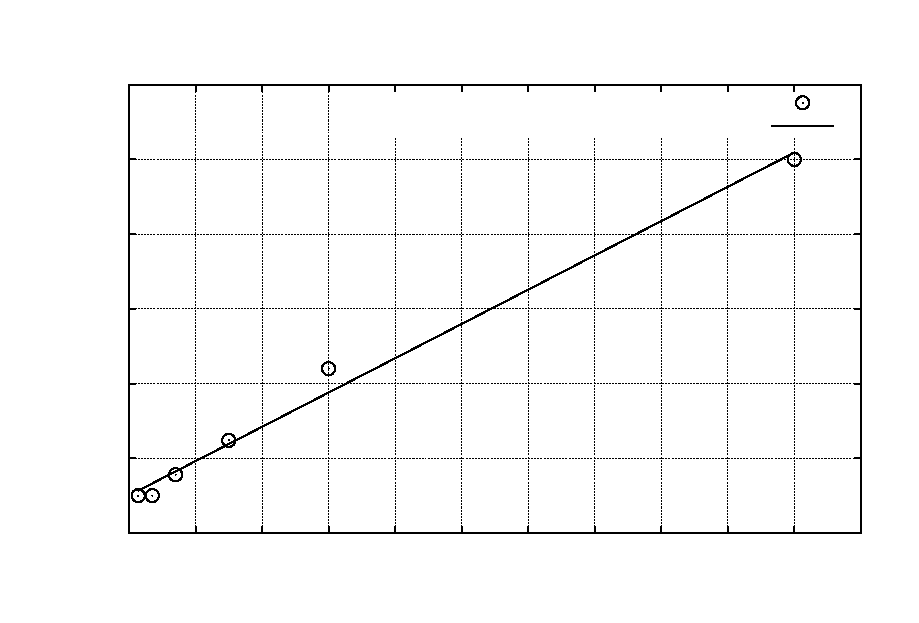
\includegraphics{fig1}}%
    \gplfronttext
  \end{picture}%
\endgroup

	\caption{Calculation time for selected datasets (labeled with roman numerals) for the 56 cores Hadoop cluster shows a linear scaling with dataset size. }
	\label{fig:fig1}
\end{figure}


\begin{figure}[!ht]
	% GNUPLOT: LaTeX picture with Postscript
\begingroup
  \makeatletter
  \providecommand\color[2][]{%
    \GenericError{(gnuplot) \space\space\space\@spaces}{%
      Package color not loaded in conjunction with
      terminal option `colourtext'%
    }{See the gnuplot documentation for explanation.%
    }{Either use 'blacktext' in gnuplot or load the package
      color.sty in LaTeX.}%
    \renewcommand\color[2][]{}%
  }%
  \providecommand\includegraphics[2][]{%
    \GenericError{(gnuplot) \space\space\space\@spaces}{%
      Package graphicx or graphics not loaded%
    }{See the gnuplot documentation for explanation.%
    }{The gnuplot epslatex terminal needs graphicx.sty or graphics.sty.}%
    \renewcommand\includegraphics[2][]{}%
  }%
  \providecommand\rotatebox[2]{#2}%
  \@ifundefined{ifGPcolor}{%
    \newif\ifGPcolor
    \GPcolorfalse
  }{}%
  \@ifundefined{ifGPblacktext}{%
    \newif\ifGPblacktext
    \GPblacktexttrue
  }{}%
  % define a \g@addto@macro without @ in the name:
  \let\gplgaddtomacro\g@addto@macro
  % define empty templates for all commands taking text:
  \gdef\gplbacktext{}%
  \gdef\gplfronttext{}%
  \makeatother
  \ifGPblacktext
    % no textcolor at all
    \def\colorrgb#1{}%
    \def\colorgray#1{}%
  \else
    % gray or color?
    \ifGPcolor
      \def\colorrgb#1{\color[rgb]{#1}}%
      \def\colorgray#1{\color[gray]{#1}}%
      \expandafter\def\csname LTw\endcsname{\color{white}}%
      \expandafter\def\csname LTb\endcsname{\color{black}}%
      \expandafter\def\csname LTa\endcsname{\color{black}}%
      \expandafter\def\csname LT0\endcsname{\color[rgb]{1,0,0}}%
      \expandafter\def\csname LT1\endcsname{\color[rgb]{0,1,0}}%
      \expandafter\def\csname LT2\endcsname{\color[rgb]{0,0,1}}%
      \expandafter\def\csname LT3\endcsname{\color[rgb]{1,0,1}}%
      \expandafter\def\csname LT4\endcsname{\color[rgb]{0,1,1}}%
      \expandafter\def\csname LT5\endcsname{\color[rgb]{1,1,0}}%
      \expandafter\def\csname LT6\endcsname{\color[rgb]{0,0,0}}%
      \expandafter\def\csname LT7\endcsname{\color[rgb]{1,0.3,0}}%
      \expandafter\def\csname LT8\endcsname{\color[rgb]{0.5,0.5,0.5}}%
    \else
      % gray
      \def\colorrgb#1{\color{black}}%
      \def\colorgray#1{\color[gray]{#1}}%
      \expandafter\def\csname LTw\endcsname{\color{white}}%
      \expandafter\def\csname LTb\endcsname{\color{black}}%
      \expandafter\def\csname LTa\endcsname{\color{black}}%
      \expandafter\def\csname LT0\endcsname{\color{black}}%
      \expandafter\def\csname LT1\endcsname{\color{black}}%
      \expandafter\def\csname LT2\endcsname{\color{black}}%
      \expandafter\def\csname LT3\endcsname{\color{black}}%
      \expandafter\def\csname LT4\endcsname{\color{black}}%
      \expandafter\def\csname LT5\endcsname{\color{black}}%
      \expandafter\def\csname LT6\endcsname{\color{black}}%
      \expandafter\def\csname LT7\endcsname{\color{black}}%
      \expandafter\def\csname LT8\endcsname{\color{black}}%
    \fi
  \fi
  \setlength{\unitlength}{0.0500bp}%
  \begin{picture}(8502.00,5668.00)%
    \gplgaddtomacro\gplbacktext{%
      \csname LTb\endcsname%
      \put(946,704){\makebox(0,0)[r]{\strut{} 1.1}}%
      \csname LTb\endcsname%
      \put(946,1319){\makebox(0,0)[r]{\strut{} 1.2}}%
      \csname LTb\endcsname%
      \put(946,1933){\makebox(0,0)[r]{\strut{} 1.3}}%
      \csname LTb\endcsname%
      \put(946,2548){\makebox(0,0)[r]{\strut{} 1.4}}%
      \csname LTb\endcsname%
      \put(946,3163){\makebox(0,0)[r]{\strut{} 1.5}}%
      \csname LTb\endcsname%
      \put(946,3778){\makebox(0,0)[r]{\strut{} 1.6}}%
      \csname LTb\endcsname%
      \put(946,4392){\makebox(0,0)[r]{\strut{} 1.7}}%
      \csname LTb\endcsname%
      \put(946,5007){\makebox(0,0)[r]{\strut{} 1.8}}%
      \csname LTb\endcsname%
      \put(1078,484){\makebox(0,0){\strut{} 0}}%
      \csname LTb\endcsname%
      \put(1956,484){\makebox(0,0){\strut{} 0.02}}%
      \csname LTb\endcsname%
      \put(2835,484){\makebox(0,0){\strut{} 0.04}}%
      \csname LTb\endcsname%
      \put(3713,484){\makebox(0,0){\strut{} 0.06}}%
      \csname LTb\endcsname%
      \put(4592,484){\makebox(0,0){\strut{} 0.08}}%
      \csname LTb\endcsname%
      \put(5470,484){\makebox(0,0){\strut{} 0.1}}%
      \csname LTb\endcsname%
      \put(6348,484){\makebox(0,0){\strut{} 0.12}}%
      \csname LTb\endcsname%
      \put(7227,484){\makebox(0,0){\strut{} 0.14}}%
      \csname LTb\endcsname%
      \put(8105,484){\makebox(0,0){\strut{} 0.16}}%
      \put(176,2855){\rotatebox{-270}{\makebox(0,0){\strut{}ratio of $F_{Hadoop}/F_{HPC}$}}}%
      \put(4591,154){\makebox(0,0){\strut{}reciprocal dataset size, 1/Gbases}}%
      \put(4591,5337){\makebox(0,0){\strut{}Figure 2}}%
    }%
    \gplgaddtomacro\gplfronttext{%
      \csname LTb\endcsname%
      \put(7578,4423){\makebox(0,0){\strut{}datasetI}}%
      \put(4240,2394){\makebox(0,0){\strut{}datasetII}}%
      \put(2747,1595){\makebox(0,0){\strut{}datasetIII}}%
      \put(1737,919){\makebox(0,0){\strut{}datasetIV}}%
      \csname LTb\endcsname%
      \put(1310,4834){\makebox(0,0)[l]{\strut{}least-squares fit to $y=aX+b$ for the data with  $b=1.13$}}%
    }%
    \gplbacktext
    \put(0,0){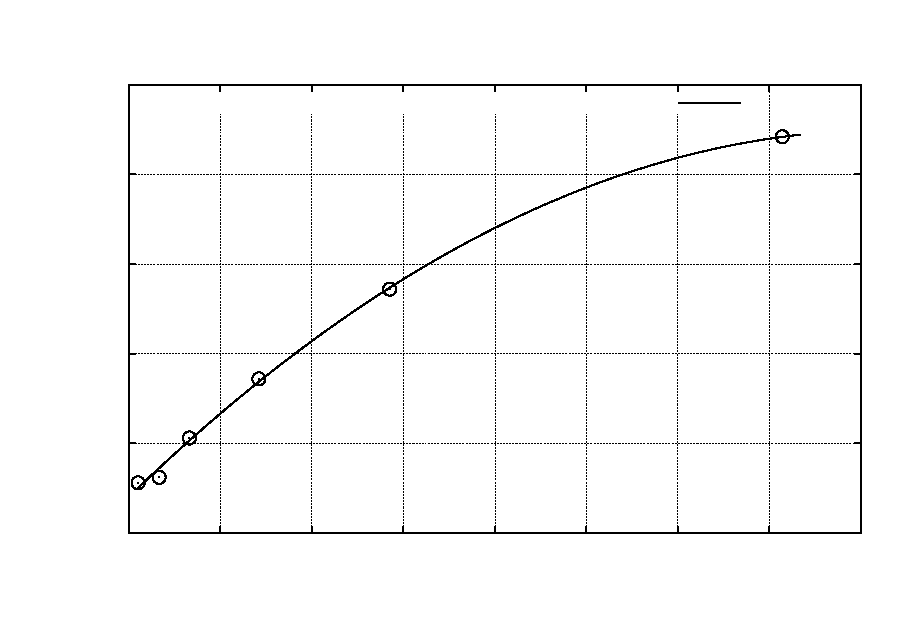
\includegraphics{fig2}}%
    \gplfronttext
  \end{picture}%
\endgroup

	\caption{The ratio of the~$F_{Hadoop}/F_{HPC}$ as a function of a reciprocal dataset size in Gbases. Calculations were carried out for 56 cores Hadoop and 16 cores HPC cluster correspondingly.
The points are fit to a quadratic least-squares curve, which makes it possible to predict {\it infinite} dataset size. Datasets are labeled with roman numerals.}
	\label{fig:fig2}
\end{figure}

\begin{figure}[!ht]
 	\begin{subfigure}[b]{0.4\textwidth}
        	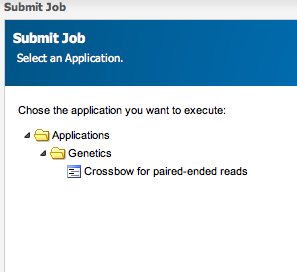
\includegraphics[width=\textwidth]{a.png}
		\subcaption{}
	\end{subfigure}
	\hspace{0.5cm}
	\begin{subfigure}[b]{0.6\textwidth}
	        	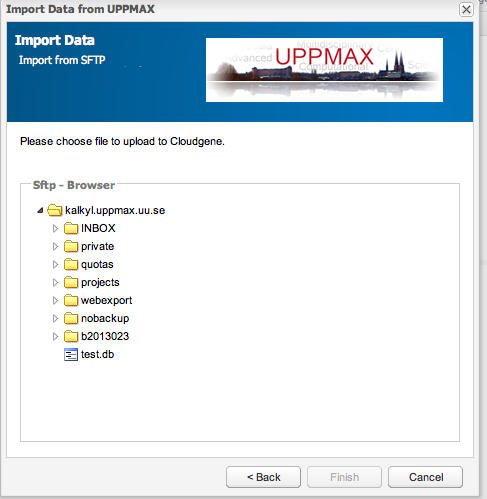
\includegraphics[width=\textwidth]{c.png}
		\subcaption{}
	\end{subfigure}
%	\begin{subfigure}[b]{0.6\textwidth}
%		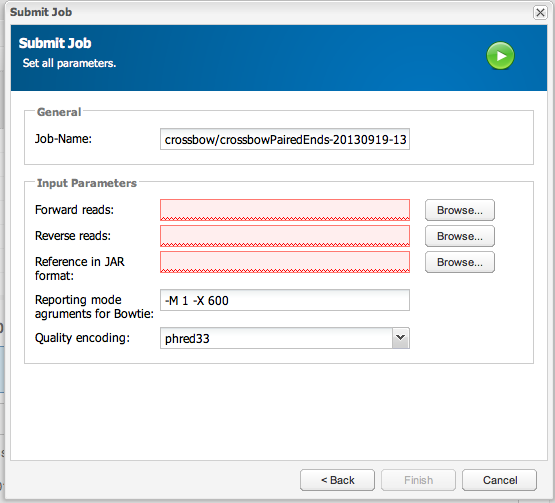
\includegraphics[width=\textwidth]{b.png}
%		\subcaption{Cloudgene: specifying job parameters}
%	\end{subfigure}
	\caption{An example of a job setup with the graphical Hadoop front-end Cloudgene, providing a smooth user experience even for novice users. \textbf{a)} Pipeline selection - in our case containing the Crossbow pipeline. \textbf{b)} The UPPMAX-adapted functionality to browsing and import data from the user's home folder in the shared file system.}
	\label{fig:fig4}
\end{figure}


\begin{figure}[!ht]
	\small
	% GNUPLOT: LaTeX picture with Postscript
\begingroup
  \makeatletter
  \providecommand\color[2][]{%
    \GenericError{(gnuplot) \space\space\space\@spaces}{%
      Package color not loaded in conjunction with
      terminal option `colourtext'%
    }{See the gnuplot documentation for explanation.%
    }{Either use 'blacktext' in gnuplot or load the package
      color.sty in LaTeX.}%
    \renewcommand\color[2][]{}%
  }%
  \providecommand\includegraphics[2][]{%
    \GenericError{(gnuplot) \space\space\space\@spaces}{%
      Package graphicx or graphics not loaded%
    }{See the gnuplot documentation for explanation.%
    }{The gnuplot epslatex terminal needs graphicx.sty or graphics.sty.}%
    \renewcommand\includegraphics[2][]{}%
  }%
  \providecommand\rotatebox[2]{#2}%
  \@ifundefined{ifGPcolor}{%
    \newif\ifGPcolor
    \GPcolorfalse
  }{}%
  \@ifundefined{ifGPblacktext}{%
    \newif\ifGPblacktext
    \GPblacktexttrue
  }{}%
  % define a \g@addto@macro without @ in the name:
  \let\gplgaddtomacro\g@addto@macro
  % define empty templates for all commands taking text:
  \gdef\gplbacktext{}%
  \gdef\gplfronttext{}%
  \makeatother
  \ifGPblacktext
    % no textcolor at all
    \def\colorrgb#1{}%
    \def\colorgray#1{}%
  \else
    % gray or color?
    \ifGPcolor
      \def\colorrgb#1{\color[rgb]{#1}}%
      \def\colorgray#1{\color[gray]{#1}}%
      \expandafter\def\csname LTw\endcsname{\color{white}}%
      \expandafter\def\csname LTb\endcsname{\color{black}}%
      \expandafter\def\csname LTa\endcsname{\color{black}}%
      \expandafter\def\csname LT0\endcsname{\color[rgb]{1,0,0}}%
      \expandafter\def\csname LT1\endcsname{\color[rgb]{0,1,0}}%
      \expandafter\def\csname LT2\endcsname{\color[rgb]{0,0,1}}%
      \expandafter\def\csname LT3\endcsname{\color[rgb]{1,0,1}}%
      \expandafter\def\csname LT4\endcsname{\color[rgb]{0,1,1}}%
      \expandafter\def\csname LT5\endcsname{\color[rgb]{1,1,0}}%
      \expandafter\def\csname LT6\endcsname{\color[rgb]{0,0,0}}%
      \expandafter\def\csname LT7\endcsname{\color[rgb]{1,0.3,0}}%
      \expandafter\def\csname LT8\endcsname{\color[rgb]{0.5,0.5,0.5}}%
    \else
      % gray
      \def\colorrgb#1{\color{black}}%
      \def\colorgray#1{\color[gray]{#1}}%
      \expandafter\def\csname LTw\endcsname{\color{white}}%
      \expandafter\def\csname LTb\endcsname{\color{black}}%
      \expandafter\def\csname LTa\endcsname{\color{black}}%
      \expandafter\def\csname LT0\endcsname{\color{black}}%
      \expandafter\def\csname LT1\endcsname{\color{black}}%
      \expandafter\def\csname LT2\endcsname{\color{black}}%
      \expandafter\def\csname LT3\endcsname{\color{black}}%
      \expandafter\def\csname LT4\endcsname{\color{black}}%
      \expandafter\def\csname LT5\endcsname{\color{black}}%
      \expandafter\def\csname LT6\endcsname{\color{black}}%
      \expandafter\def\csname LT7\endcsname{\color{black}}%
      \expandafter\def\csname LT8\endcsname{\color{black}}%
    \fi
  \fi
  \setlength{\unitlength}{0.0500bp}%
  \begin{picture}(8502.00,5668.00)%
    \gplgaddtomacro\gplbacktext{%
      \csname LTb\endcsname%
      \put(946,704){\makebox(0,0)[r]{\strut{} 0}}%
      \put(946,1242){\makebox(0,0)[r]{\strut{} 0.5}}%
      \put(946,1780){\makebox(0,0)[r]{\strut{} 1}}%
      \put(946,2318){\makebox(0,0)[r]{\strut{} 1.5}}%
      \put(946,2856){\makebox(0,0)[r]{\strut{} 2}}%
      \put(946,3393){\makebox(0,0)[r]{\strut{} 2.5}}%
      \put(946,3931){\makebox(0,0)[r]{\strut{} 3}}%
      \put(946,4469){\makebox(0,0)[r]{\strut{} 3.5}}%
      \put(946,5007){\makebox(0,0)[r]{\strut{} 4}}%
      \put(1078,484){\makebox(0,0){\strut{} 0}}%
      \put(2483,484){\makebox(0,0){\strut{} 0.05}}%
      \put(3889,484){\makebox(0,0){\strut{} 0.1}}%
      \put(5294,484){\makebox(0,0){\strut{} 0.15}}%
      \put(6700,484){\makebox(0,0){\strut{} 0.2}}%
      \put(8105,484){\makebox(0,0){\strut{} 0.25}}%
      \put(176,2855){\rotatebox{-270}{\makebox(0,0){\strut{}$T_{mapping}/T_{comm}$}}}%
      \put(4591,154){\makebox(0,0){\strut{}reciprocal number of nodes, $1/N$}}%
      \put(4591,5337){\makebox(0,0){\strut{}Ratios of the  short reads mapping time per node to the communication  time}}%
    }%
    \gplgaddtomacro\gplfronttext{%
      \csname LTb\endcsname%
      \put(7118,1977){\makebox(0,0)[r]{\strut{}HPC SLURM}}%
      \csname LTb\endcsname%
      \put(7118,1757){\makebox(0,0)[r]{\strut{}Hadoop}}%
      \csname LTb\endcsname%
      \put(7118,1537){\makebox(0,0)[r]{\strut{}HPC random}}%
      \csname LTb\endcsname%
      \put(7118,1317){\makebox(0,0)[r]{\strut{}linear fit for Hadoop }}%
      \csname LTb\endcsname%
      \put(7118,1097){\makebox(0,0)[r]{\strut{}linear fit for HPC SLURM}}%
      \csname LTb\endcsname%
      \put(7118,877){\makebox(0,0)[r]{\strut{}linear fit for HPC random}}%
    }%
    \gplbacktext
    \put(0,0){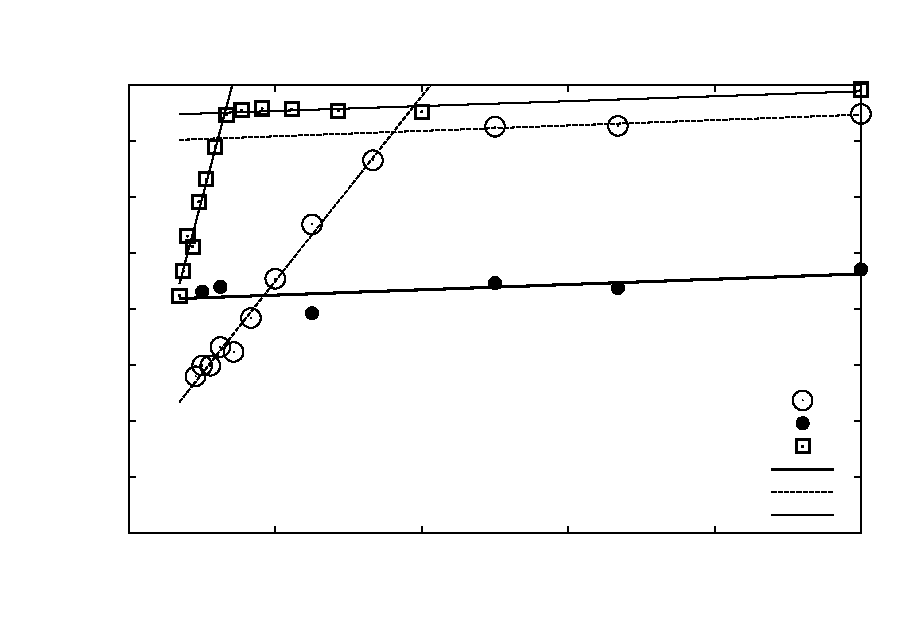
\includegraphics{fig3}}%
    \gplfronttext
  \end{picture}%
\endgroup

	\normalsize
	\caption{Ratios of the alignment time~$T_{alignment}$ to the communication costs~$T_{comm}$ for HPC and Hadoop clusters for Dataset~IV as a function of reciprocal number of nodes~$1/N$. Two HPC scenarios are shown as ``HPC SLURM'' and ``HPC random'', which correspond to standard SLURM behavior and a modified one where nodes are being allocated from random racks.
Linear fit  to $ax+b$ was done with the least-squares method.
The estimated values for Hadoop approach are $(a,b)\approx(0.95,2.07)$.
One  can see two defined linear regions for the HPC approach with very different tangents for linear and non-linear scalings correspondingly.
For  the ``HPC SLURM'' $(a,b)\approx (0.96, 3.49)$ and $(a,b)\approx (32.99, 0.60)$, and for  the ``HPC random'' $(a,b)\approx (0.88, 3.72)$ and $(a,b)\approx (98.24, 0.53)$.
 The constant term for HPC goes below unity, i.e. for the large number of nodes the communication will take more time than actual alignment. 
%The first one resembles to that of Hadoop, and corresponds to the case then the communication in the cluster is not a bottleneck. 
%The second one shows the regime corresponding to the case of saturation of the network, resulting in traffic jams: data distibution time~$T_{comm}$ stops to scale 
%linearly to the reciprocal cluster size, and becomes more of less a constant, while the alignment time continues to satisfy~$T_{alignment}\propto 1/N$.
}
	\label{fig:fig3}
\end{figure}







%%%%%%%%%%%
% Tables
%%%%%%%%%%%
\section*{Tables}

 \begin{table}[hbtp]
\small

\caption{Timings (in minutes) for the sort routine of the Samtools package for the dataset IV (58 Gbases BAM file). The measurements are done on a single HPC node with $p=16$ cores. Averaging is done over 5 independent simulations. The amount of RAM is given for all 16 cores. }
\begin{center}
\begin{tabular}{|l|c|c|c|c|c|c|c|}
RAM, GB		&	8			&		16			&			32		& 		64				\\
timing, minutes	&	$208\pm50$	&	$172\pm13$		&	$136\pm12$		& 	$87\pm11$			\\
\end{tabular}
\end{center}
\label{table:5}
\normalsize
\end{table}%




\begin{table}[!ht]
\small
\caption{Timings (in minutes) with Crossbow's native read preprocessor and with derived approach for  datasets II, III, IV  on a 56 cores Hadoop cluster, using the Crossbow, and with the BASH script on a single HPC node with 16 cores.}
\begin{center}
\begin{tabular}{l|c|c|c}
Dataset			&		II (7 Gbases )	& III (30 Gbases)	& IV (100 Gbases)\\
\hline
Crossbow native			&		$60.6\pm0.7$	& $299.0\pm2.3$	&	$673\pm1.0$	\\
Hadoop, this work			&		$7.0\pm0.0$	&	$20.7\pm0.4$&		$52.4\pm0.1$\\
BASH, this work			& 		$7.4\pm0.0$	&	$31.1\pm0.1$	&	$114.5\pm0.3$	\\
\end{tabular}
\end{center}
\label{table:preprocess}
\normalsize
\end{table}%


\begin{table}[!ht]
\small
\caption{Timings for Dataset I processed on different number of cores of a HPC node.}
\begin{center}
\begin{tabular}{c|c|c|c|ccc}
$N$ cores	&\multicolumn{3}{c|}{timing, minutes}&\multicolumn{3}{c}{speed-ups} \\
\hline
	& alignment 	&	SNP calling	&	total  &total & alignment& SNP call\\
\hline
1	&	22.75	$\pm$1.24&	26.1$\pm$0.7	&	48.9	&	 1.00	&	1.00	&	1.00\\
2	&	11.00$\pm$0.05	&	16.9$\pm$1.3	&	27.9	&	 0.88	&	1.03	&	0.77\\
4	&	5.91$\pm$0.04	&	11.7$\pm$0.5	&	17.6	&	 0.69	&	0.96	&	0.56\\
6	&	4.24$\pm$0.04	&	8.6$\pm$0.8	&	12.8	&	 0.64	&	0.89	&	0.51\\
8	&	3.44$\pm$0.03	&	8.6$\pm$0.9	&	12.1	&	 0.51	&	0.83	&	0.38\\
10	&	2.91$\pm$0.01	&	7.7$\pm$0.5	&	10.6	&	 0.46	&	0.78	&	0.34\\
12	&	2.64$\pm$0.04	&	7.5$\pm$0.5	&	10.1	&	 0.40	&	0.72	&	0.29\\
14	&	2.57$\pm$0.03	&	7.5$\pm$0.6	&	10.1	&	 0.35	&	0.63	&	0.25\\
16	&	2.88$\pm$0.06	&	7.4$\pm$0.4	&	10.2	&	 0.30	&	0.49	&	0.22\\
\end{tabular}
\end{center}
\label{table:3}
\normalsize
\end{table}


\begin{table}[!ht]
\small

\caption{Timings  (in minutes) for HPC and  Hadoop deployments for different dataset sizes.    Dataset are labelled by roman numerals, ``f.r.'' stands for ``forward reads''. The large variance for the HPC deployment is due to Samtools BAM sorting, which is IO and memory intensive, thus strongly depend on the queuing at the HPC cluster.}
\begin{center}
\begin{tabular}{l|c|c|c|c|c|c|c}

data, Gbases		&	1.4	&	3.5		&	7.0		&	15.0		&	30.0		&	100.0	&	250 	\\
				&	(I)	&	(II, f.r.)	&	(II)		&	(III, f.r.)	&	(III)		&	(IV)		&	(V)\\
\hline
Hadoop, 56 cores&--&	--	&39		&62	&108	&250&1125\\
Hadoop, 56 cores		&	$18\pm0	$	&	$18\pm0	$	&	$29\pm0$	&	$47\pm0	$	&	$89\pm0$	&	$238\pm1$		&	$1164\pm14$\\
HPC1, 8 cores&	41&	96	&157	&307	&596	&1490&--\\
HPC, 16 cores	&	$17\pm1$	&	$22\pm6$	&	$43\pm3$	&	$81\pm9$	&	$172\pm15$		&	$467\pm60$	& $>48$ hours\\

\end{tabular}
\end{center}
\label{table:4}
\normalsize
\end{table}%


\begin{table}[!ht]
\small
\footnotesize
\caption{Datasets used in the comparison. }
\begin{center}
\begin{tabular}{|l|l|l|}
dataset &	organism &	size in Gbases\\
\hline
 I		&	{\it A.thaliana}	&	1.4	\\
 II	&	{\it A.thaliana}	&	7.0\\
  III	&	{\it A.thaliana}	&	30.0	\\
 IV	&{\it A.thaliana}, the artificial dataset created using Samtools package	&	100.0	\\
 V	&	{\it H.sapiens}, two individuals (GM12750 and GM12004), sample SRR499924		&	250.0\\

\end{tabular}
\end{center}
\label{table:datasets}
\normalsize
\end{table}%


\begin{table}[!ht]
\caption{Timings  for alignment and the ratio~$T_{alignment}/T_{comm}$ for HPC and Hadoop clusters for Dataset IV.
For the ``HPC random'' approach, data chunks have to be copied to the local scratch disks first and the alignments (SAM files) copied back while Hadoop keeps all the data inside HDFS and hence does not need data staging. Hadoop however needs to preprocess reads before the actual alignment stage in order to be able to operate in MR manner resulting in what we term ``communication costs''. Note that each HPC node has 16 cores, while each Hadoop node has 7 (one core is dedicated to run the virtual machine).}
\begin{center}
\begin{tabular}{c|c|c|c|c|c}
 \multicolumn{3}{c|}{Hadoop} & \multicolumn{3}{c}{ HPC random} \\
 \hline		


Number of nodes	&Alignment time,	&$\frac{T_{alignment}}{T_{comm}}$	&Number of nodes	&Alignment time,	&$\frac{T_{alignment}}{T_{comm}}$\\
(cores)					&minutes		&							&(cores)			&minutes&\\
\hline
4(28)	&293.5	&2.33	&4(64)	&74.4	&3.89\\
6(42)	&189.8	&2.19	&10(160)	&32.4	&3.76\\
8(56)	&136.0	&2.23	&14(224)	&22.7	&3.77\\
16(112)	&70.3	&1.96	&18(288)	&17.9	&3.78\\
32(224)	&39.3	&2.20	&22(352)	&14.5	&3.79\\
40(280)	&32.5	&2.15	&26(416)	&12.3	&3.77\\
			&&&30(480)	&10.7	&3.73\\
			&&&34(544)	&9.5	&3.45\\
			&&&38(608)	&8.5	&3.16\\
			&&&42(672)	&7.6	&2.96\\
			&&&46(736)	&7.0	&2.55\\
			&&&50(800)	&6.4	&2.65\\
			&&&54(864)	&5.9	&2.34\\
			&&&58(928)	&5.5	&2.12\\

\end{tabular}
\end{center}
\label{table:6}
\end{table}%





\end{document}

